\newpage
\section{Normal Forms Around Periodic Orbits} \label{sec:NormalForms}

Normal form theory provides a systematic way to simplify a non-linear dynamical system near an invariant object through a suitable change of coordinates. 
The central idea is to apply a sequence of near-identity transformations that remove non-essential non-linear terms while retaining the dominant structure of the dynamics. 
For Hamiltonian systems, such as the CR3BP, these transformations must be symplectic so that the Hamiltonian structure of the original system is preserved. 
The resulting simplified system is advantageous because its dynamics can be described analytically, enabling closed-form propagation in the transformed coordinates. 
As a result, the long-term evolution of objects near a periodic orbit can be approximated in a single evaluation rather than through computationally expensive numerical integration over many years or decades. 
This capability is particularly useful for applications such as predicting the evolution of space debris in the cislunar domain over long time-horizons. 
In the following, we provide an overview of normal form theory in the context of periodic orbits in the CR3BP and present numerical results demonstrating its application.

\subsection{Normal Form Theory}
This section provides only a concise overview of the normal form transformations used in this work; a more complete theoretical description can be found in Sinha's dissertation \cite{Sinha2026}. 
The methodology follows the numerical normal form framework developed by Jorba and Villanueva \cite{Jorba1998,Jorba1999}. 
The implementation used in the present analysis was developed with contributions from Sinha \cite{Sinha2026} and is applied here to the examples considered below. 
We describe the transformations at a high level and emphasize how the Hamiltonian changes at each step.
For a Hamiltonian $H$, the equations of motion in canonical coordinates can be written as
\begin{equation}
    \dot{\boldsymbol{x}} = \boldsymbol{J} \nabla H(\boldsymbol{x}), \qquad
    \boldsymbol{J} = \begin{pmatrix}
    0 & I \\
    - I & 0
    \end{pmatrix},
\end{equation}
where $\boldsymbol{J}$ is the canonical symplectic matrix. 
The coordinate transformations used below are symplectic, meaning that they preserve this canonical Hamiltonian structure.

Let the periodic orbit be denoted by $\boldsymbol{\gamma}:\mathbb{R}\rightarrow\mathbb{R}^6$, with $\boldsymbol{\gamma}(t+T)=\boldsymbol{\gamma}(t)$. 
The first step in constructing the normal form is to translate the periodic orbit to the origin using
\begin{equation}
    \boldsymbol{\xi}=\boldsymbol{x}-\boldsymbol{\gamma}(t).
\end{equation}
The Hamiltonian in the translated coordinates, denoted by $K_1(t,\boldsymbol{\xi})$, is time dependent. 
Expanding about $\boldsymbol{\xi}=0$ gives
\begin{equation}
K_1(t,\boldsymbol{\xi})
=
\frac{1}{2}\boldsymbol{\xi}^{T}
\nabla^2 H(\boldsymbol{\gamma}(t))
\boldsymbol{\xi}
+
\sum_{d \geq 3} H_d^{(\boldsymbol{\xi})}(t,\boldsymbol{\xi}),
\end{equation}
where $\nabla^2 H(\boldsymbol{\gamma}(t))$ is the Hessian of the original Hamiltonian evaluated along the periodic orbit, and $H_d^{(\boldsymbol{\xi})}$ denotes the homogeneous polynomial terms of degree $d$ in $\boldsymbol{\xi}$. 
The constant and linear terms vanish because the expansion is taken about the translated periodic solution.

The next transformation removes the explicit time dependence from the quadratic part of the Hamiltonian. 
This is achieved through a Floquet transformation to new coordinates $\boldsymbol{\eta}$,
\begin{equation}
    \boldsymbol{\eta}=\boldsymbol{P}^{-1}(t)\boldsymbol{\xi}.
\end{equation}
Here, $\boldsymbol{P}(t)$ is the periodic part of the STM decomposition
\begin{equation}
\label{eq: STM decomposition}
\boldsymbol{\Phi}(t) = \boldsymbol{P}(t)e^{t\boldsymbol{B}},
\end{equation}
where $\boldsymbol{P}(t+T)=\boldsymbol{P}(t)$ and $\boldsymbol{P}(0)=\boldsymbol{I}$. 
The matrix $\boldsymbol{\Phi}(t)$ is the STM of the variational dynamics in the translated $\boldsymbol{\xi}$ coordinates, defined in the same sense as Eq. \eqref{eq: STM} and $\boldsymbol{B}$ is a Floquet exponent matrix. 
Once $\boldsymbol{B}$ is determined from
\begin{equation}
    \boldsymbol{B} = \frac{1}{T}\log\!\left(\boldsymbol{\Phi}(T)\right),
\end{equation}
the periodic matrix $\boldsymbol{P}(t)$ follows from \cref{eq: STM decomposition}. 
In Floquet coordinates, the Hamiltonian takes the form
\begin{equation}
    K_2(t,\boldsymbol{\eta}) 
    = \frac{1}{2}\boldsymbol{\eta}^{\top} \boldsymbol{S} \boldsymbol{\eta} 
    + \sum_{d \ge 3} H_d^{(\boldsymbol{\eta})}(t,\boldsymbol{\eta}),
\end{equation}
where the quadratic part is now autonomous and $\boldsymbol{S}=-\boldsymbol{J}\boldsymbol{B}$.

The remaining transformations remove higher-order nonresonant terms from the Hamiltonian. 
At each degree $d$, this is done by solving the homological equation
\begin{equation}
    \label{eq: homological equation}
    \mathcal{L}_d W_d + Z_d = H_d^{(\boldsymbol{\eta})}.
\end{equation}
Here, $W_d(t,\boldsymbol{\eta})$ is the generating function of the near-identity transformation, and $Z_d$ contains the terms that remain in the normal form. 
Ideally, $W_d$ is chosen so that $Z_d=0$; however, terms that lie in the kernel of the homological operator cannot be removed and are retained as resonant terms. 
The homological operator is defined as
\begin{equation}
    \mathcal{L}_d W 
    \equiv \partial_t W + \{ W, H_2 \}, 
    \qquad 
    \{ W, H_2 \} \equiv \nabla W^{\top} J \nabla H_2,
\end{equation}
where $H_2=\frac{1}{2}\boldsymbol{\eta}^{\top}\boldsymbol{S}\boldsymbol{\eta}$ is the quadratic Hamiltonian.

Since the higher-order terms remain time periodic, they can be expanded in a Fourier series,
\begin{equation}
    H_d^{(\boldsymbol{\eta})}(t,\boldsymbol{\eta})
    =
    \sum_{|k|\le K} H_{d,k}(\boldsymbol{\eta}) e^{ik\omega t},
    \qquad 
    \omega = \frac{2\pi}{T},
\end{equation}
where the series is truncated at Fourier order $K$. 
Expanding $W_d$ and $Z_d$ in the same form decouples the homological equation by polynomial degree and Fourier mode, allowing the normal form transformation to be computed term by term.

The final Hamiltonian consists of the autonomous quadratic part together with the resonant higher-order terms that cannot be removed. 
It defines the approximate dynamics in the normal form coordinates $\boldsymbol{u}$, in which objects can be propagated analytically.

\subsection{Numerical Results}

We test the normal form construction using a planar Lyapunov orbit around the libration point $\mathcal{L}_1$. 
The orbit is shown in \cref{fig:ex_lyap} together with its Floquet multipliers, defined as the eigenvalues of the monodromy matrix. 
Because the orbit lies in a region where the gravitational influence of both the Earth and the Moon is significant, its dynamics are highly unstable, as indicated by the multiplier far outside the unit circle. 
This instability makes the orbit a challenging test case for the normal form approximation.

\begin{figure}[t!]
    \centering
    \begin{subfigure}{0.29\textwidth}
        \centering
        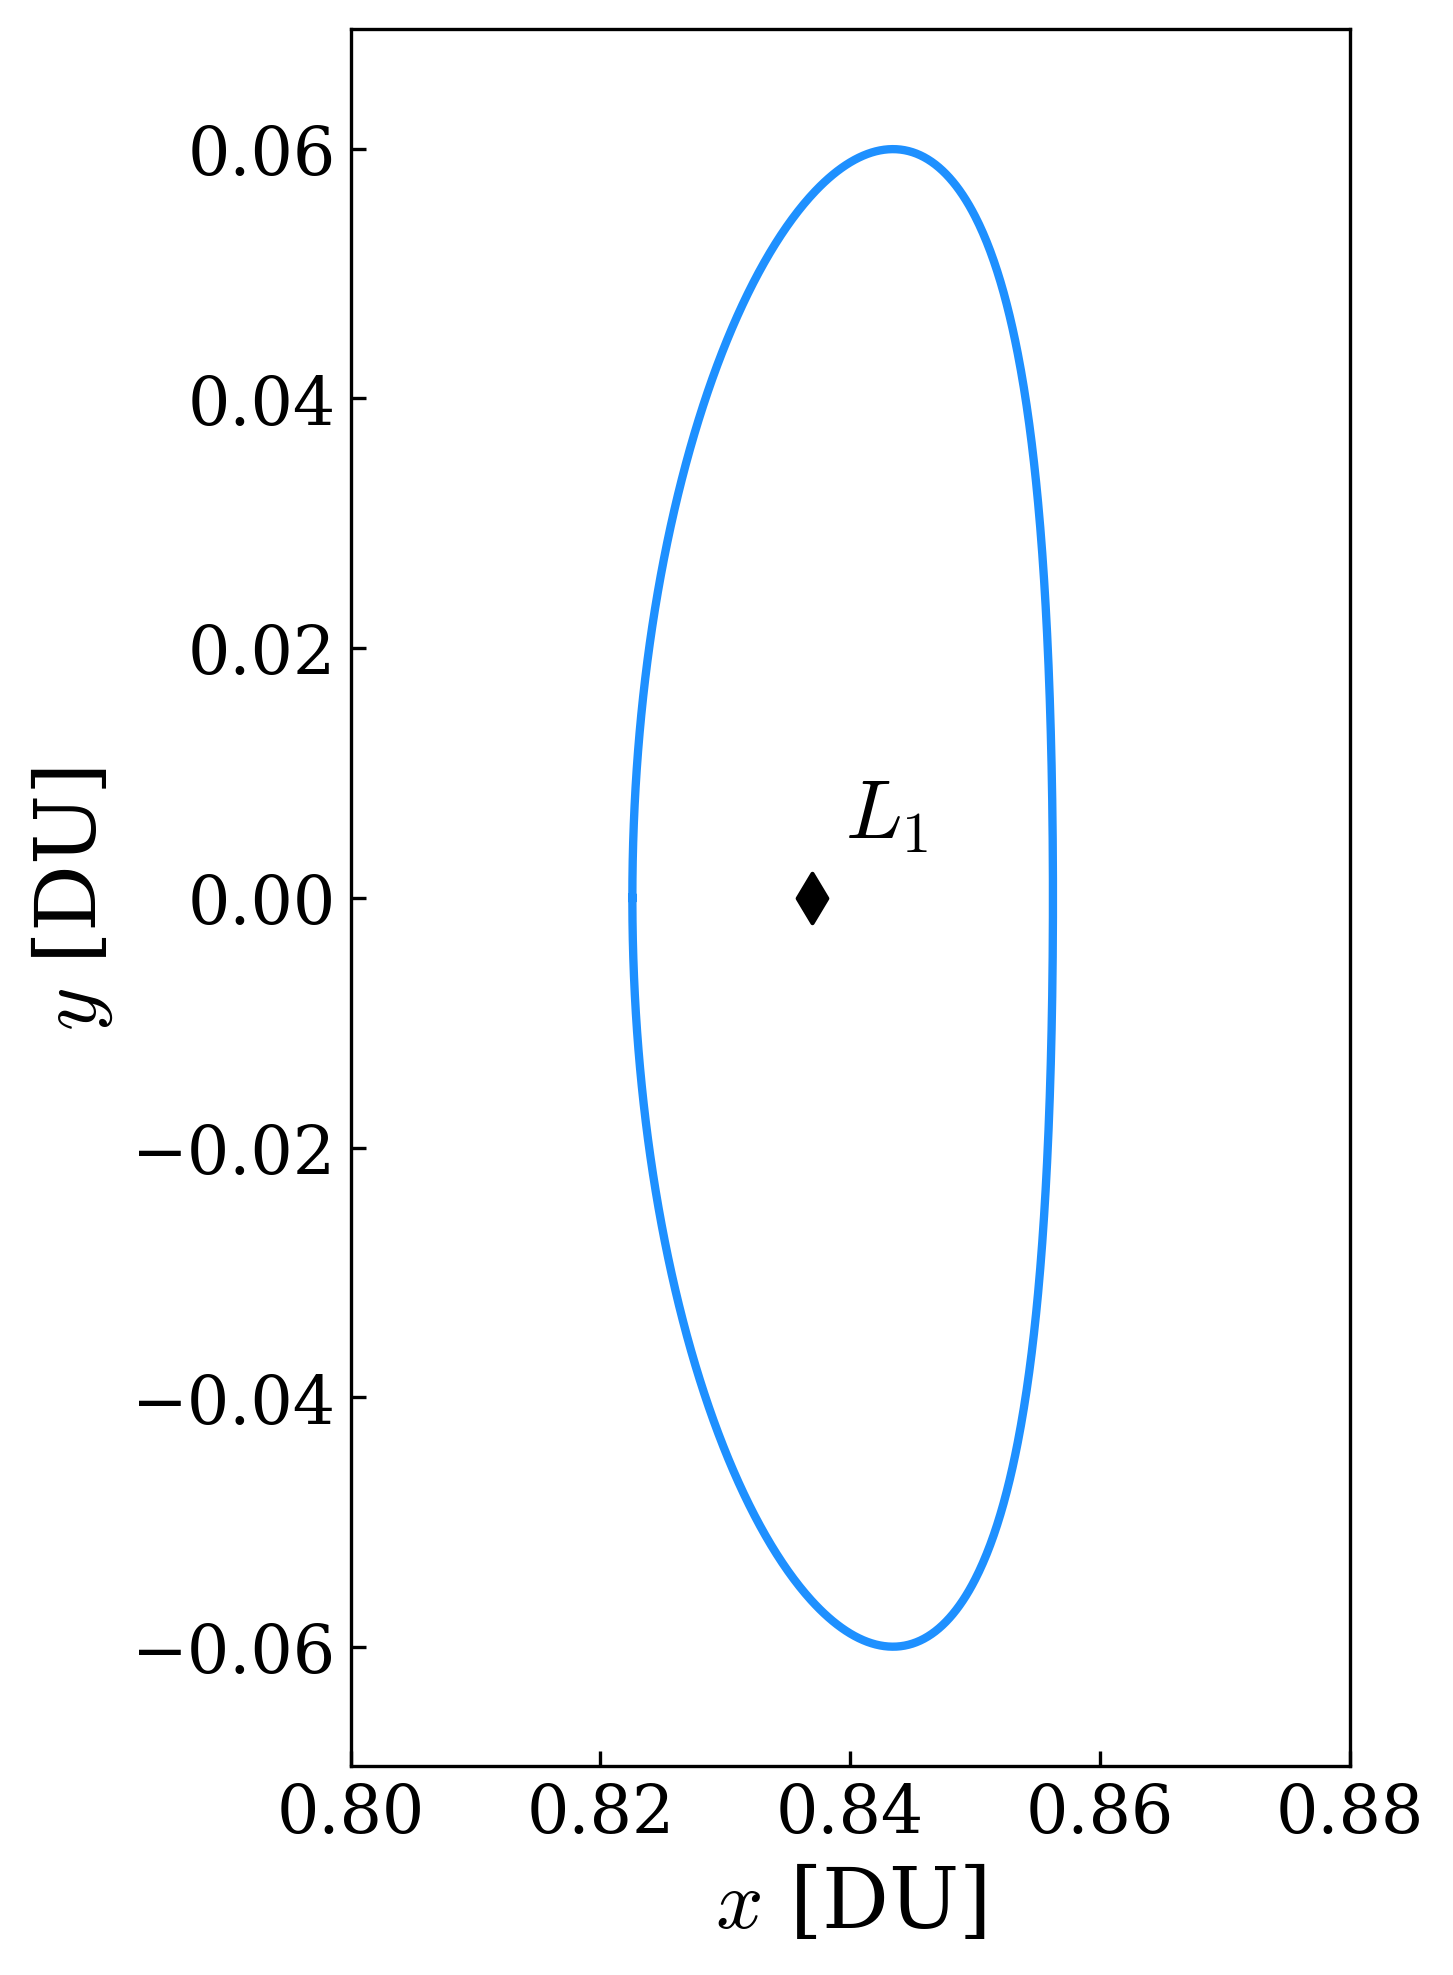
\includegraphics[height=6.3cm,keepaspectratio]{images/lyapunov_orbit_xy.png}
        \caption{Trajectory in $x$-$y$.}
        \label{fig:traj}
    \end{subfigure}
    \hfill
    \begin{subfigure}{0.69\textwidth}
        \centering
        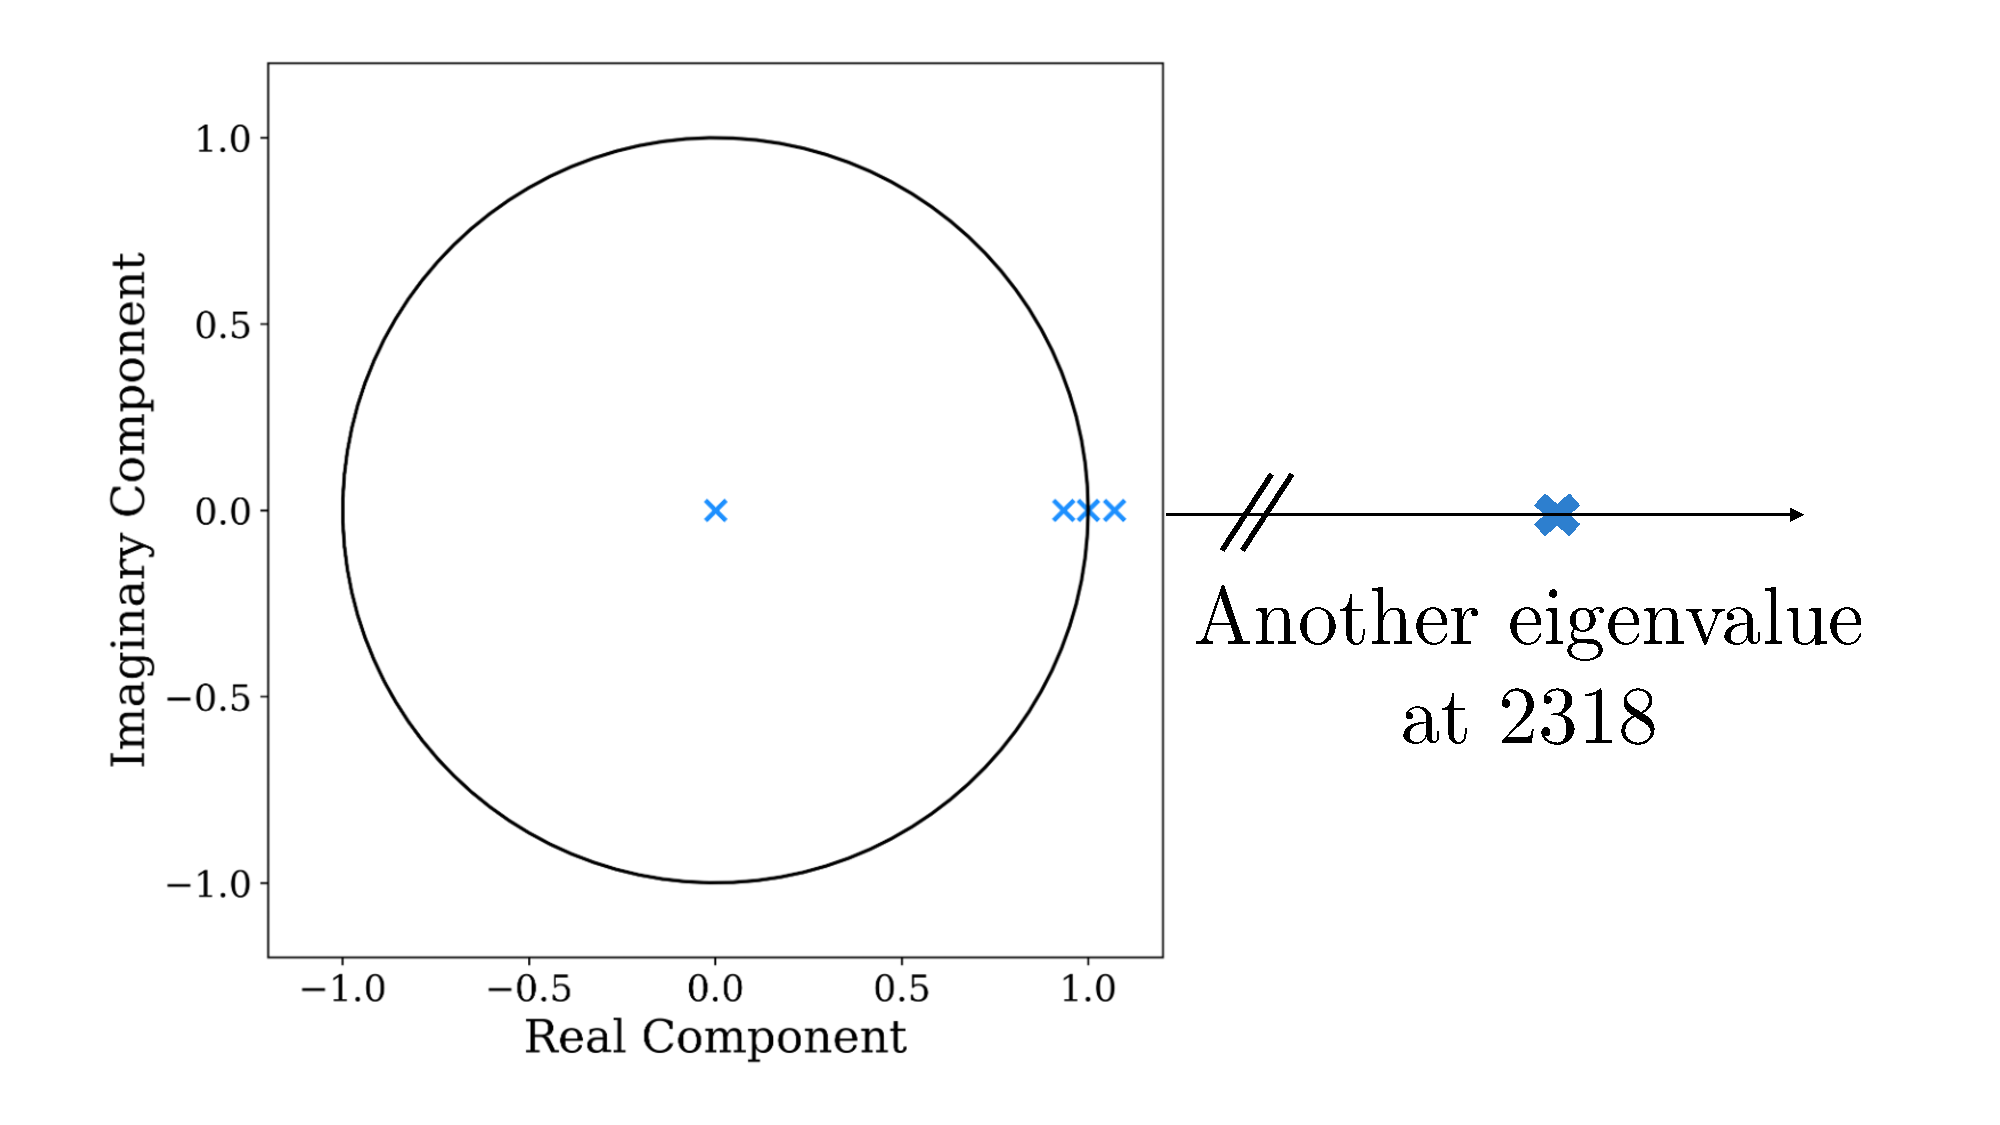
\includegraphics[height=6.3cm,keepaspectratio]{images/floquet_plot.pdf}
        \caption{Floquet multipliers in the complex plane.}
        \label{fig:floq}
    \end{subfigure}

    \caption{Planar Lyapunov orbit used to test the normal form construction.}
    \label{fig:ex_lyap}
\end{figure}

To demonstrate the application of the normal form, we initialize a set of nearby trajectories from a Gaussian distribution centered on the Lyapunov orbit and propagate them using both the full synodic CR3BP dynamics and the simplified normal form system. 
The initial Gaussian is sampled on the Poincaré section $y=0$ around the initial crossing point of the Lyapunov orbit. 
The standard deviations are chosen as 
$\sigma_x = 10^{-6}\,\mathrm{DU}\,(384\,\mathrm{m})$, 
$\sigma_{v_x} = 10^{-4}\,\mathrm{VU}\,(0.1\,\mathrm{m}/\mathrm{s})$, and
$\sigma_{v_y} = 10^{-4}\,\mathrm{VU}\,(0.1\,\mathrm{m}/\mathrm{s})$.
We draw $100$ samples from this distribution and map each sample to normal form coordinates using the transformations $\boldsymbol{x}\rightarrow\boldsymbol{u}$ described above. 
To limit the computational cost, the normal form is truncated at polynomial degree $D=4$, and the time-periodic coefficients are represented using a Fourier expansion of order $K=16$. 
The samples are then propagated analytically in normal form coordinates for one orbital period. 
For comparison, the same initial conditions are propagated in the synodic CR3BP coordinates using an adaptive step-size RK54 integrator. 
To compare both propagation methods, the analytically propagated normal form trajectories are mapped back to the synodic frame through the inverse transformation $\boldsymbol{u}\rightarrow\boldsymbol{x}$ at the same time instances used by the numerical integrator. 
The results are shown in \cref{fig:nf_comparison}.

\begin{figure}[b!]
    \centering
    \begin{subfigure}{0.39\textwidth}
        \centering
        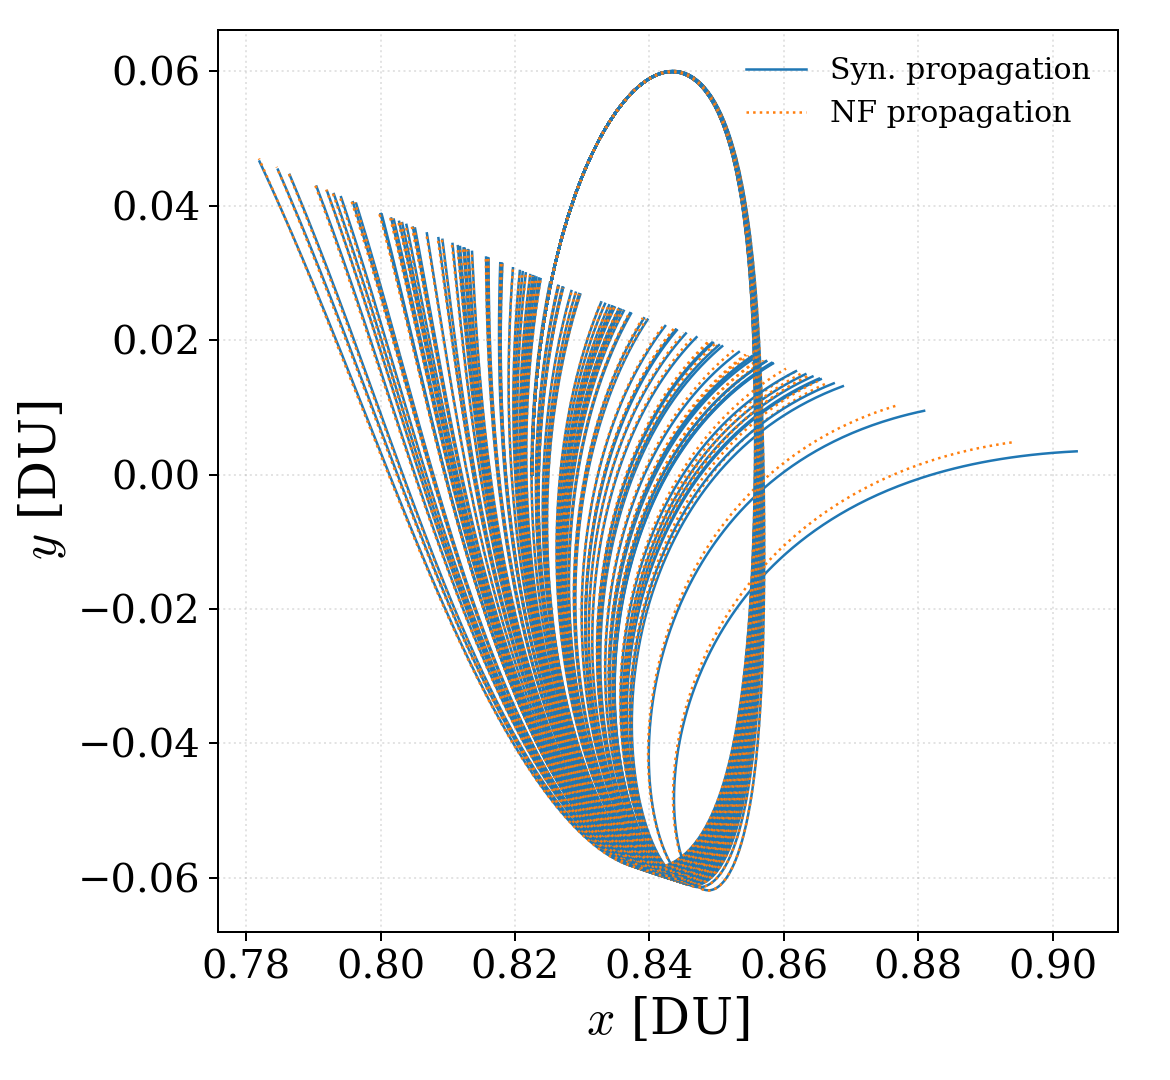
\includegraphics[height=5.3cm,keepaspectratio]{images/propagation_test_1_synodic_comparison_xy.png}
        \caption{Trajectories in $x$-$y$ space.}
        \label{fig:nf_traj}
    \end{subfigure}
    \hfill
    \begin{subfigure}{0.59\textwidth}
        \centering
        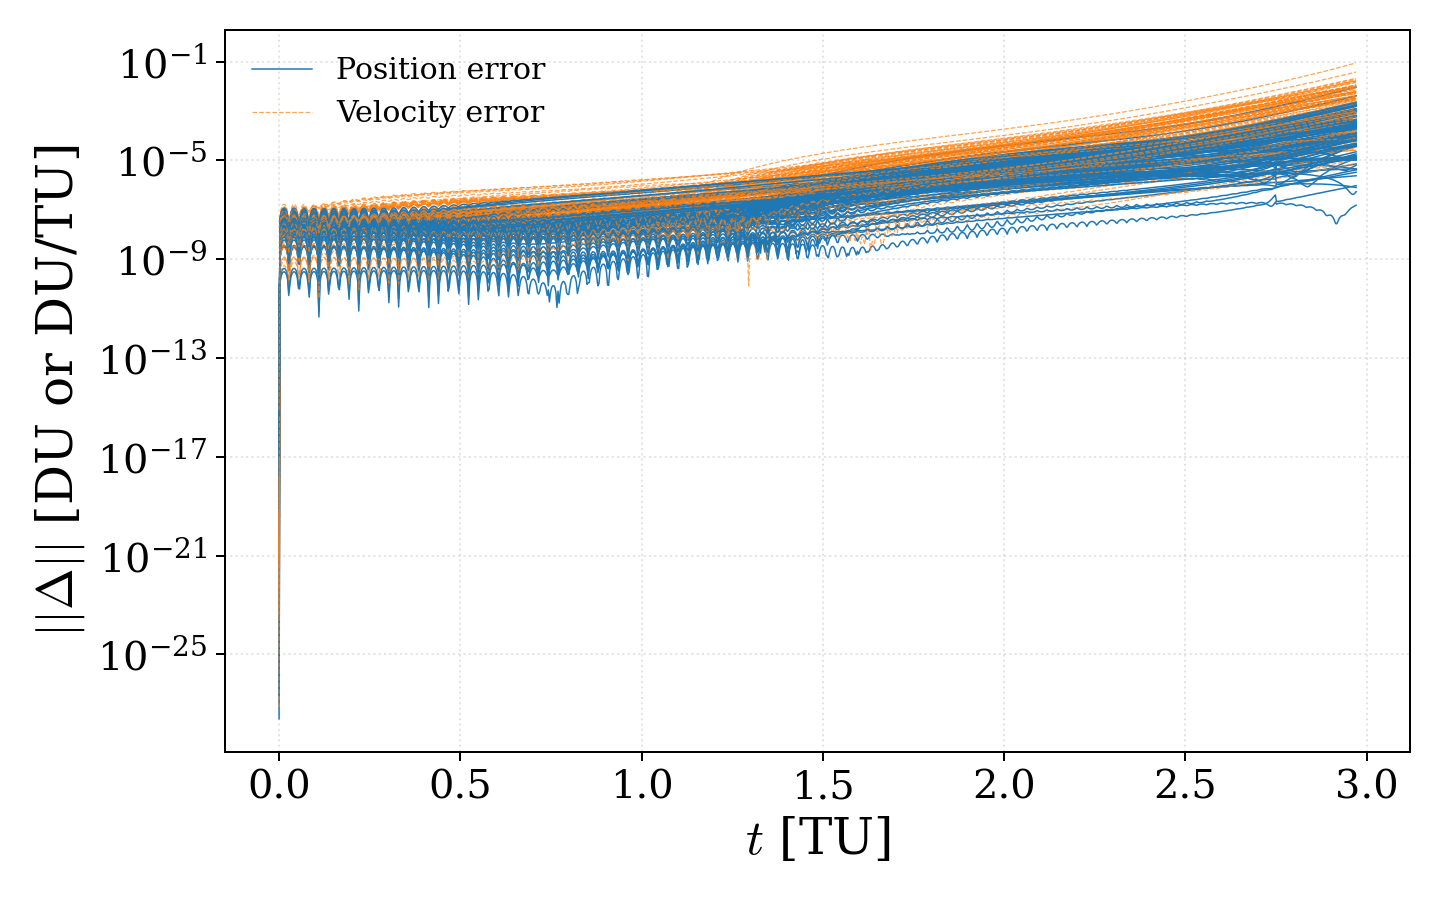
\includegraphics[height=5.3cm,keepaspectratio]{images/propagation_test_1_synodic_error.png}
        \caption{Position and velocity errors.}
        \label{fig:nf_err}
    \end{subfigure}

    \caption{Comparison of propagation in synodic and normal form coordinates.}
    \label{fig:nf_comparison}
\end{figure}

The left panel of \cref{fig:nf_comparison} compares the trajectories obtained with both propagation methods in the $x$-$y$ plane. 
Despite the small initial perturbations, the trajectories depart rapidly from the reference orbit over one period due to the strong instability of the Lyapunov orbit. 
Nevertheless, the normal form propagation closely follows the full synodic propagation while the trajectories remain near the reference orbit. 
As the trajectories move farther away, the accuracy decreases because the normal form is a local approximation; however, it still captures the qualitative behavior of the perturbed trajectories. 
This behavior is also reflected in the right panel, which shows the $L_2$ norms of the position and velocity errors over time for all propagated trajectories.